\documentclass[a4paper, 12pt]{scrartcl}
\usepackage[assign-num=3]{report}

\title{Comparison of Game Engines}

\begin{document}

\maketitle

\section{Introduction}
A game engine is a tool for developers of video games. It is software framework which abstracts away core parts of a video game such as rendering, physics, input handling, sound, AI, etc. It typically includes software libraries and other software in the form of a software development kit (SDK), which contains additional tools revolving around the engine's ecosystem (level editor, asset packager, and so on).

A game engine enables developers to create games more efficiently, since a lot of the fundamental components of a game are available for use out of the box. This saves developers the time of having to implement all these core features from scratch, which could otherwise add a tremendous amount of complexity to the project. For example, game engines may offer cross-platform capabilities in a more or less transparent way to the developers. This removes the necessity to deal with the plethora of different platform-specific APIs, which allows developers and publishers to reach a broader market more easily.

\subsection{History}
Game engines were not immediately prevalent in the industry when it first started. This is because the platforms were much more fragmented, and there was little standardisation (and thus little compatibility) among them. Furthermore, hardware was being developed at a rapid pace. All these factors made it difficult to re-use any abstractions (such as those provided by a game engine) in the long term. Hardware was also quite limited, so it was necessary to build a game's components from scratch and custom-tailor them to the target platform to ensure the game ran optimally.

The earliest software that may constitute a game engine was in-house for use with first-party software. These engines were far more limited in scope than modern game engines (what may now be considered \textit{middleware} used by a game engine). Engines for third-parties became prevalent in the 1990s along with the growing popularity and feasibility of 3D graphics. This led to influential engines such as id Tech and Unreal Engine, which are in some form or another still in use with modern games.

Such engines were developed for first-party games, but made available for licensing to third-party developers. Companies shifted their strategy to developing the game and its engine separately. This decoupling enabled the engine to be usable by third parties, and allowed developers to become more specialised.

\section{Comparing Source and Unity}
This section compares and contrasts various aspects of two different engines: Source by Valve Software and Unity by Unity Technologies.

\subsection{Development Environment}
\subsubsection{Source}
Programming is done in C++, typically using Visual Studio. However, other IDEs can also work. A level editor named \textit{Hammer} is included in the Source SDK. When not programming or making assets, this is tool that is being worked with the most. It is used to define the level's geometry, apply textures, light the level, place objects and entities, configure behaviour logic for entities, and much more.

\begin{figure}[!htp]
  \centering
  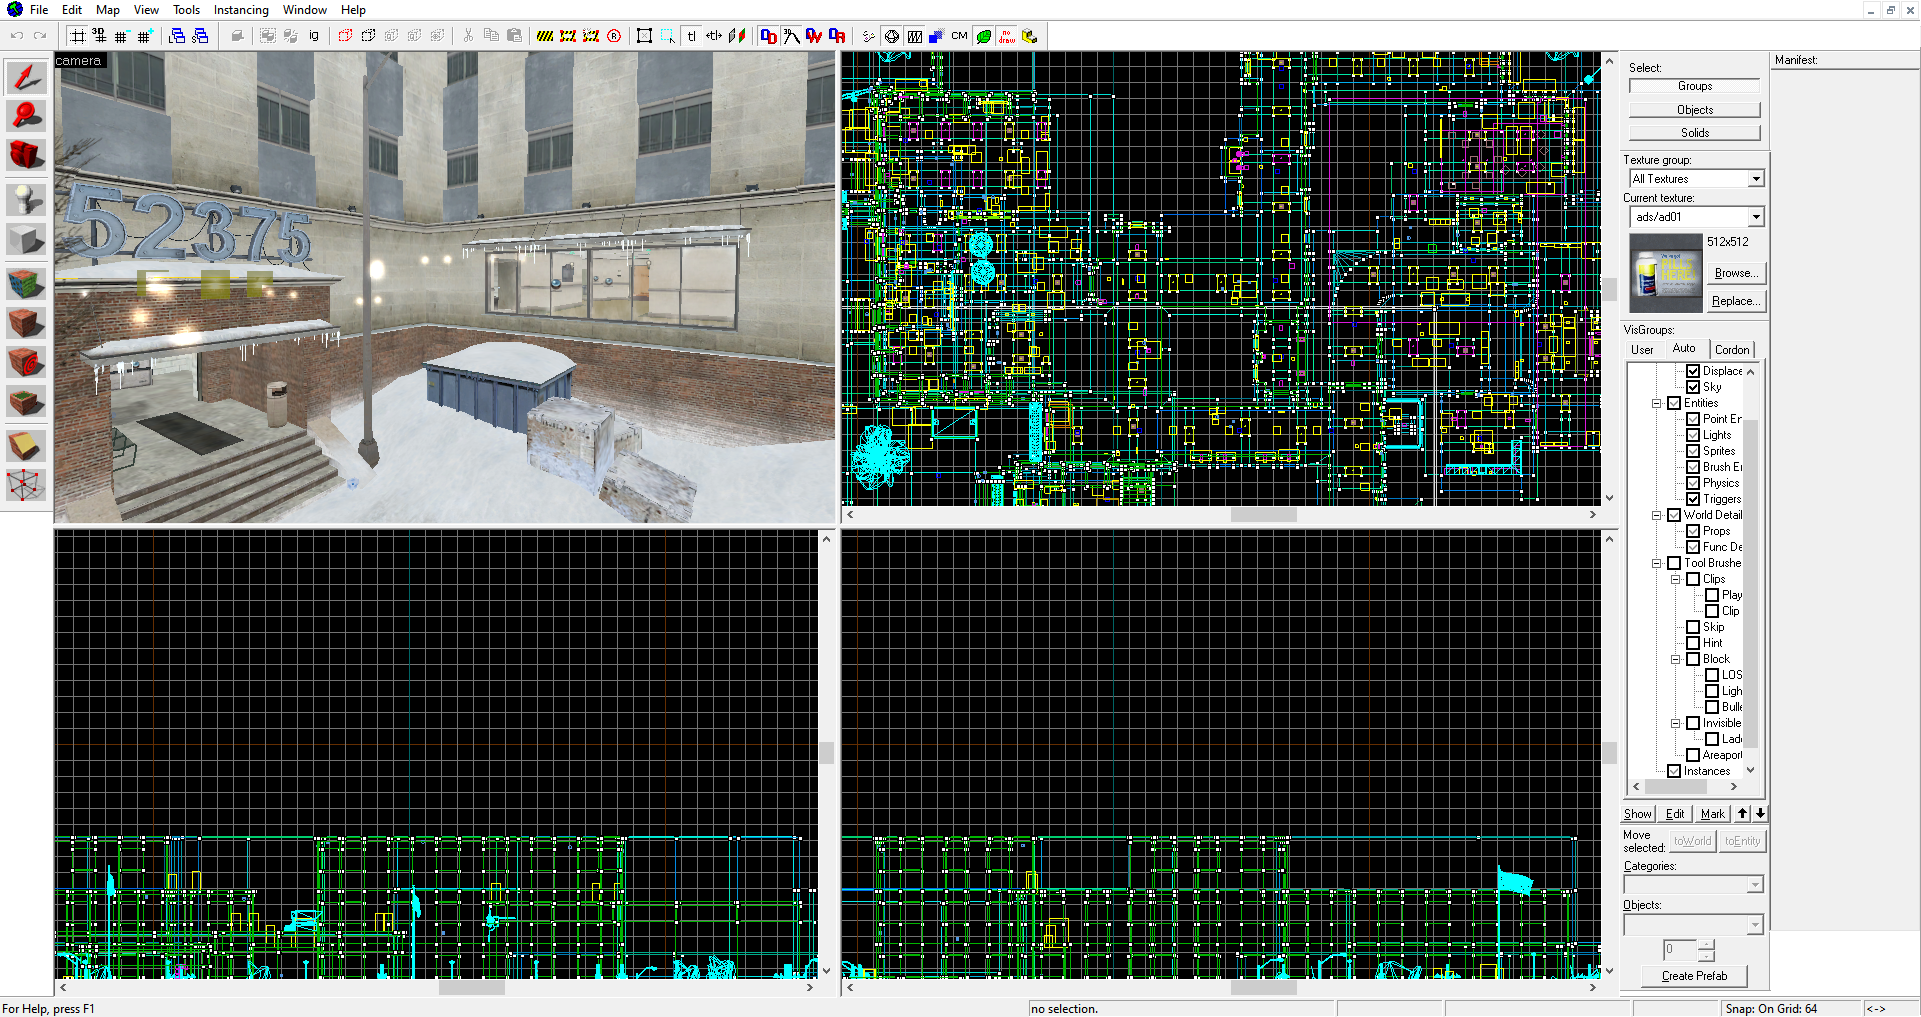
\includegraphics[width=\linewidth]{images/source_hammer.png}
  \caption{Hammer editing \textit{cs\_office} from CS:GO}
\end{figure}

Assets such as models and textures are expected to be created using third-party tools. For modelling, Autodesk XSI and Maya were historically popular. However, it's more common these days to use one of the third-party plugins for other modelling tools such as Blender.

Some assets, including models and textures, are expected to be in Source-specific formats. To achieve this, the Source SDK provides some command-line tools to convert assets to the expected formats. For example, \texttt{vtex} is used for texture conversion and \texttt{studiomdl} is used to compile models. There are various other command-line tools, like \texttt{vbsp}, \texttt{vvis}, and \texttt{vrad} for map compilation and \texttt{vpk} for packaging game assets.

There are also third-party tools frequently used by modders and level designers, such as VIDE, which can be used to create textures, view or create game content packages, edit particles, pack game content into map files, and much more.

\begin{figure}[!htp]
  \centering
  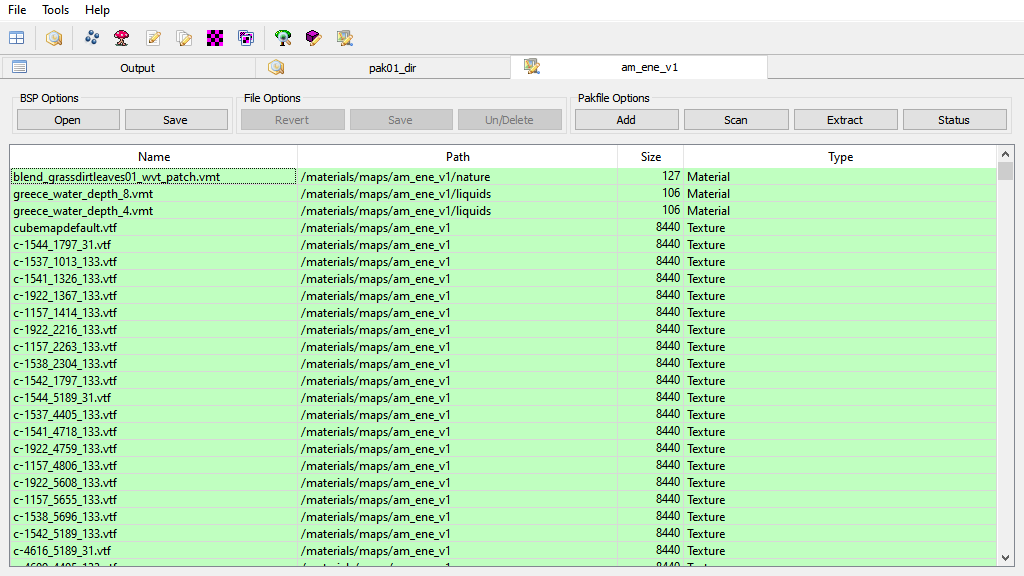
\includegraphics[width=\linewidth]{images/source_vide_pakfile.png}
  \caption{VIDE displaying the pakfile lump of a map}
\end{figure}

\paragraph{Unity}

\end{document}
